\documentclass{AISB2008}
\usepackage{listings}

\lstset{
  xleftmargin=.35\columnwidth, xrightmargin=.35\columnwidth
}

\usepackage{times}
\usepackage{graphicx}
\usepackage{latexsym}

\usepackage{amsmath}

\makeatletter
\renewcommand{\boxed}[1]{\text{\fboxsep=.2em\fbox{\m@th$\displaystyle#1$}}}
\makeatother

\usepackage{amsopn}
\newcommand{\droparrow}{%
  \mathchoice{\raisebox{-4pt}{$\displaystyle\mapsto$}}
             {\raisebox{-4pt}{$\mapsto$}}
             {\raisebox{-2pt}{$\scriptstyle\mapsto$}}
             {\raisebox{-2pt}{$\scriptscriptstyle\mapsto$}}}

\usepackage{marvosym,hetcasl}


\usepackage[hidelinks]{hyperref}

\begin{document}

\title{The Search for Computational Intelligence,\\ or, How Universal is Universality?}

\author{Joseph Corneli\institute{Department of Computing, Goldsmiths College, University of London\newline\Email \url{j.corneli@gold.ac.uk}} \and Ewen Maclean\institute{School of Informatics, University of Edinburgh\newline\Email \url{ewenmaclean@gmail.com}} }

\maketitle
\bibliographystyle{AISB2008}

\begin{abstract}
XXX YYY
\end{abstract}

\section{Introduction}

\begin{figure}
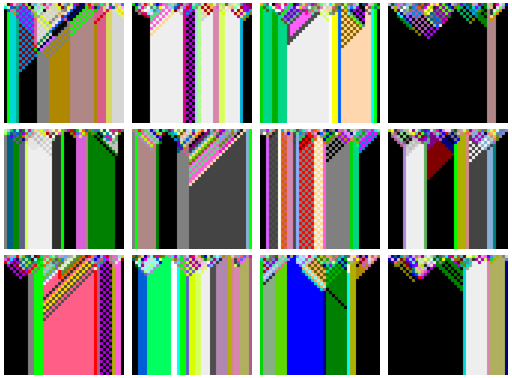
\includegraphics[width=\columnwidth]{metaca.png}
\caption{An illustration of MetaCA evolution}
\end{figure}

This paper takes a local approach to studying the
evolution of cellular automata, following on the
global approach of \cite{pavlic2014self}.

\newpage

\section{Background}

\cite{mitchell1993revisiting} is the classic work on ``edge of
chaos.'' (Read more here and talk about the $\lambda$ thing.)

\cite{hofstadter1995prolegomena,marshall1999metacat} took a rather
different but still somewhat related approach.


Explain the background on computational blending and why we thought
domain would be a revealing experiment.  (Basically, CAs do a simple
kind of blending already.)

\subsection{Conceptual Blending}

Following the approach of Goguen \cite{}, we propose exploiting
existing formalisms of blending in the context of cellular automata to
investigate emergent and novel behaviours. The fundamental building blocks used in calculating concept or theory blends are
\begin{description}
\item[Input Concepts] are the theories or concepts which have some degree of commonality, which is not necessarily syntactic. 
\item[Signature Morphism] is a definition of how symbols are mapped between theories or concepts. 
\item[Generic Space] is the space which contains a theory which is common to both input theories.
\item[Blend] is the space computed by combining both theories. The computation is computed using a ``pushout'' from the underlying categorical semantics \cite{}. 
\end{description}

Once a blend has been computed, it may represent a concept which is in some way inconsistent. Equally it may represent a concept which is in some way incomplete. We can then either weaken an input teory or refine the blend:
\begin{description}
\item[Weakening] Given an inconsistent blend it is possible to weaken the input concept in order to produce a consistent blend. Weakening means removing symbols or axioms from the input concept.
\item[Refinement] Given a blend which represents a concept which is in some way incomplete, it is possible to refine the concept by adding symbols or axioms.
\end{description}

This paper presents an example of concepts to which the blending process applies. We describe the components of blending in the context of cellular automata in \S\ref{}.

\clearpage

\section{Implementation}
%%%% describe genotype/phenotype definition?


%%%% section header?
\subsection{Generating Genotypes}

To explain how this works, consider the following example.  Each elementary CA rule defines a mapping from all eight strings of 0's and 1's to the set \{0,1\}.  Thus, for example the rule 01010100 is defined as the following operation:
\begin{lstlisting}[mathescape]
0 0 0 $\mapsto$ 0
0 0 1 $\mapsto$ 1
0 1 0 $\mapsto$ 0
1 0 0 $\mapsto$ 1
0 1 1 $\mapsto$ 0
1 0 1 $\mapsto$ 1
1 1 0 $\mapsto$ 0
1 1 1 $\mapsto$ 0
\end{lstlisting}

There are 256 of these rules. So, we can build a CA with 256 colors, rather than the traditional 2, and make the state of any given cell a ``rule''. Then we can apply this rule to decide the output for the next cell, depending on the neighbours. For example, since the middle column in the top half of the diagram below is the rule described above, we can apply this rule to each of the rows in order to produce the result in the bottom half:
\begin{lstlisting}[mathescape]
0 $\mathbf{0}$ 0     $0$ 
1 $\mathbf{1}$ 1     $0$ 
1 $\mathbf{0}$ 0     $1$
0 $\mathbf{1}$ 1  $\droparrow$   $0$
1 $\mathbf{0}$ 0     $1$ 
1 $\mathbf{1}$ 1     $0$ 
1 $\mathbf{0}$ 0     $1$ 
0 $\mathbf{0}$ 1     $1$ 
\end{lstlisting}

This is the straightforward application of a rule without any blending per se, and the results are not particularly impressive.  If we do this with blending, there’s one more step, and we get a different result.

%%%introduce blending
\subsection{Introducing Blending}

%%% say what the input concepts are - call them input rules

The blending variant says to first compute the ``generic space'' by looking at places where the two adjacent neighbours are the same. Then, whereever we have not resolved the ambiguity (indicated by $\ast$), apply the local rule, as above, to compute the final result: 01101101 in this case.

\lstset{
  xleftmargin=.3\columnwidth, xrightmargin=.3\columnwidth
}

\begin{lstlisting}[mathescape]
0 $\mathbf{0}$ 0     0     $\:0$
1 $\mathbf{1}$ 1     1     $\:1$
1 $\mathbf{0}$ 0     *     $\boxed{1}$
0 $\mathbf{1}$ 1  $\droparrow$   *  $\droparrow$   $\boxed{0}$
1 $\mathbf{0}$ 0     *     $\boxed{1}$
1 $\mathbf{1}$ 1     1     $\:1$
1 $\mathbf{0}$ 0     *     $\boxed{1}$
0 $\mathbf{0}$ 1     *     $\boxed{1}$
\end{lstlisting}

This blend is formalised in the HETS system \cite{} by introducing CASL files to represent the 8 bit encodings:
%%%
%%% CASL file stuff
%%%
The computed blend is inconsistent as there is not a unique value representing the output value of each function. In order to resolve this we weaken the input rules in CASL by removing the function values which cause conflict. We now have:






%%%% below is the CASL latex
\begin{figure}[!ht]
\begin{hetcasl}
\KW{library} \Id{metaca}\\
\\
\KW{logic} \SId{CASL}\\
\\
\SPEC \=\SIdIndex{METACABitencoding} \Ax{=}\\
\> \KW{free} \KW{type} \=\Id{Bit} \Ax{:}\Ax{:}\=\Ax{=} \Ax{0} \AltBar{} \Ax{1}\\
\> \SORT \Id{Triple}\\
\> \OPS \=\Id{t} \Ax{:} \=\Id{Bit} \Ax{\times} \Id{Bit} \Ax{\times} \Id{Bit} \Ax{\rightarrow} \Id{Triple};\\
\>\> \Id{bitop}\Ax{\_\_} \Ax{:} \=\Id{Triple} \Ax{\rightarrow} \Id{Bit}\\
\KW{end}\\
\\
\SPEC \=\SIdIndex{LeftRule} \Ax{=}\\
\> \SId{METACABitencoding}\\
\THEN \=\Ax{\bullet} \=\Id{bitop} \Id{t}(\=\Ax{0}, \Ax{0}, \Ax{0}) \Ax{=} \Ax{0}\\
\> \Ax{\bullet} \=\Id{bitop} \Id{t}(\=\Ax{0}, \Ax{0}, \Ax{1}) \Ax{=} \Ax{1}\\
\> \Ax{\bullet} \=\Id{bitop} \Id{t}(\=\Ax{0}, \Ax{1}, \Ax{0}) \Ax{=} \Ax{1}\\
\> \Ax{\bullet} \=\Id{bitop} \Id{t}(\=\Ax{0}, \Ax{1}, \Ax{1}) \Ax{=} \Ax{0}\\
\> \Ax{\bullet} \=\Id{bitop} \Id{t}(\=\Ax{1}, \Ax{0}, \Ax{0}) \Ax{=} \Ax{1}\\
\> \Ax{\bullet} \=\Id{bitop} \Id{t}(\=\Ax{1}, \Ax{0}, \Ax{1}) \Ax{=} \Ax{1}\\
\> \Ax{\bullet} \=\Id{bitop} \Id{t}(\=\Ax{1}, \Ax{1}, \Ax{0}) \Ax{=} \Ax{1}\\
\> \Ax{\bullet} \=\Id{bitop} \Id{t}(\=\Ax{1}, \Ax{1}, \Ax{1}) \Ax{=} \Ax{0}\\
\KW{end}\\
\\
\SPEC \=\SIdIndex{RightRule} \Ax{=}\\
\> \SId{METACABitencoding}\\
\THEN \=\Ax{\bullet} \=\Id{bitop} \Id{t}(\=\Ax{0}, \Ax{0}, \Ax{0}) \Ax{=} \Ax{0}\\
\> \Ax{\bullet} \=\Id{bitop} \Id{t}(\=\Ax{0}, \Ax{0}, \Ax{1}) \Ax{=} \Ax{1}\\
\> \Ax{\bullet} \=\Id{bitop} \Id{t}(\=\Ax{0}, \Ax{1}, \Ax{0}) \Ax{=} \Ax{0}\\
\> \Ax{\bullet} \=\Id{bitop} \Id{t}(\=\Ax{0}, \Ax{1}, \Ax{1}) \Ax{=} \Ax{1}\\
\> \Ax{\bullet} \=\Id{bitop} \Id{t}(\=\Ax{1}, \Ax{0}, \Ax{0}) \Ax{=} \Ax{0}\\
\> \Ax{\bullet} \=\Id{bitop} \Id{t}(\=\Ax{1}, \Ax{0}, \Ax{1}) \Ax{=} \Ax{1}\\
\> \Ax{\bullet} \=\Id{bitop} \Id{t}(\=\Ax{1}, \Ax{1}, \Ax{0}) \Ax{=} \Ax{0}\\
\> \Ax{\bullet} \=\Id{bitop} \Id{t}(\=\Ax{1}, \Ax{1}, \Ax{1}) \Ax{=} \Ax{1}\\
\KW{end}\\
\\
\SPEC \=\SIdIndex{LocalRule} \Ax{=}\\
\> \SId{METACABitencoding}\\
\THEN \=\Ax{\bullet} \=\Id{bitop} \Id{t}(\=\Ax{0}, \Ax{0}, \Ax{0}) \Ax{=} \Ax{0}\\
\> \Ax{\bullet} \=\Id{bitop} \Id{t}(\=\Ax{0}, \Ax{0}, \Ax{1}) \Ax{=} \Ax{1}\\
\> \Ax{\bullet} \=\Id{bitop} \Id{t}(\=\Ax{0}, \Ax{1}, \Ax{0}) \Ax{=} \Ax{0}\\
\> \Ax{\bullet} \=\Id{bitop} \Id{t}(\=\Ax{0}, \Ax{1}, \Ax{1}) \Ax{=} \Ax{1}\\
\> \Ax{\bullet} \=\Id{bitop} \Id{t}(\=\Ax{1}, \Ax{0}, \Ax{0}) \Ax{=} \Ax{0}\\
\> \Ax{\bullet} \=\Id{bitop} \Id{t}(\=\Ax{1}, \Ax{0}, \Ax{1}) \Ax{=} \Ax{1}\\
\> \Ax{\bullet} \=\Id{bitop} \Id{t}(\=\Ax{1}, \Ax{1}, \Ax{0}) \Ax{=} \Ax{0}\\
\> \Ax{\bullet} \=\Id{bitop} \Id{t}(\=\Ax{1}, \Ax{1}, \Ax{1}) \Ax{=} \Ax{0}\\
\KW{end}\\
\\
\SPEC \=\SIdIndex{Generic} \Ax{=}\\
\> \SId{METACABitencoding}\\
\THEN \=\Ax{\bullet} \=\Id{bitop} \Id{t}(\=\Ax{0}, \Ax{0}, \Ax{0}) \Ax{=} \Ax{0}\\
\> \Ax{\bullet} \=\Id{bitop} \Id{t}(\=\Ax{0}, \Ax{0}, \Ax{1}) \Ax{=} \Ax{1}\\
\> \Ax{\bullet} \=\Id{bitop} \Id{t}(\=\Ax{1}, \Ax{0}, \Ax{1}) \Ax{=} \Ax{1}\\
\KW{end}\\
\\
\VIEW \=\SId{Left} \Ax{:} \=\SId{Generic} \KW{to} \SId{LeftRule}\\
\KW{end}\\
\\
\VIEW \=\SId{Right} \Ax{:} \=\SId{Generic} \KW{to} \SId{RightRule}\\
\KW{end}\\
\\
\SPEC \=\SIdIndex{Blend} \Ax{=}\\
\> \KW{combine} \=\Id{Left}, \Id{Right}\\
\KW{end}\\
\\
\SPEC \=\SIdIndex{WeakenedLeftRule} \Ax{=}\\
\> \SId{METACABitencoding}\\
\THEN \=\Ax{\bullet} \=\Id{bitop} \Id{t}(\=\Ax{0}, \Ax{0}, \Ax{0}) \Ax{=} \Ax{0}\\
\> \Ax{\bullet} \=\Id{bitop} \Id{t}(\=\Ax{0}, \Ax{0}, \Ax{1}) \Ax{=} \Ax{1}\\
\> \Ax{\bullet} \=\Id{bitop} \Id{t}(\=\Ax{0}, \Ax{1}, \Ax{0}) \Ax{=} \Ax{1}\\
\> \Ax{\bullet} \=\Id{bitop} \Id{t}(\=\Ax{0}, \Ax{1}, \Ax{1}) \Ax{=} \Ax{0}\\
\> \Ax{\bullet} \=\Id{bitop} \Id{t}(\=\Ax{1}, \Ax{0}, \Ax{0}) \Ax{=} \Ax{1}\\
\> \Ax{\bullet} \=\Id{bitop} \Id{t}(\=\Ax{1}, \Ax{0}, \Ax{1}) \Ax{=} \Ax{1}\\
\> \Ax{\bullet} \=\Id{bitop} \Id{t}(\=\Ax{1}, \Ax{1}, \Ax{0}) \Ax{=} \Ax{1}\\
\KW{end}\\
\\
\SPEC \=\SIdIndex{WeakenedRightRule} \Ax{=}\\
\> \SId{METACABitencoding}\\
\THEN \=\Ax{\bullet} \=\Id{bitop} \Id{t}(\=\Ax{0}, \Ax{0}, \Ax{0}) \Ax{=} \Ax{0}\\
\> \Ax{\bullet} \=\Id{bitop} \Id{t}(\=\Ax{0}, \Ax{0}, \Ax{1}) \Ax{=} \Ax{1}\\
\> \Ax{\bullet} \=\Id{bitop} \Id{t}(\=\Ax{1}, \Ax{0}, \Ax{1}) \Ax{=} \Ax{1}\\
\> \Ax{\bullet} \=\Id{bitop} \Id{t}(\=\Ax{1}, \Ax{1}, \Ax{1}) \Ax{=} \Ax{1}\\
\KW{end}\\
\\
\VIEW \=\SId{WeakenedLeft} \Ax{:} \=\SId{Generic} \KW{to} \SId{WeakenedLeftRule}\\
\KW{end}\\
\\
\VIEW \=\SId{WeakenedRight} \Ax{:} \=\SId{Generic} \KW{to} \SId{WeakenedRightRule}\\
\KW{end}\\
\\
\SPEC \=\SIdIndex{ConsistentBlend} \Ax{=}\\
\> \KW{combine} \=\Id{WeakenedLeft}, \Id{WeakenedRight}\\
\KW{end}
\end{hetcasl}
\end{figure}


(Say more about Baldwin effect, mutations, and Game of Life
simulator.)

We've put the working code on Github\footnote{\url{https://github.com/holtzermann17/metaca}}. 


\newpage

\begin{figure}
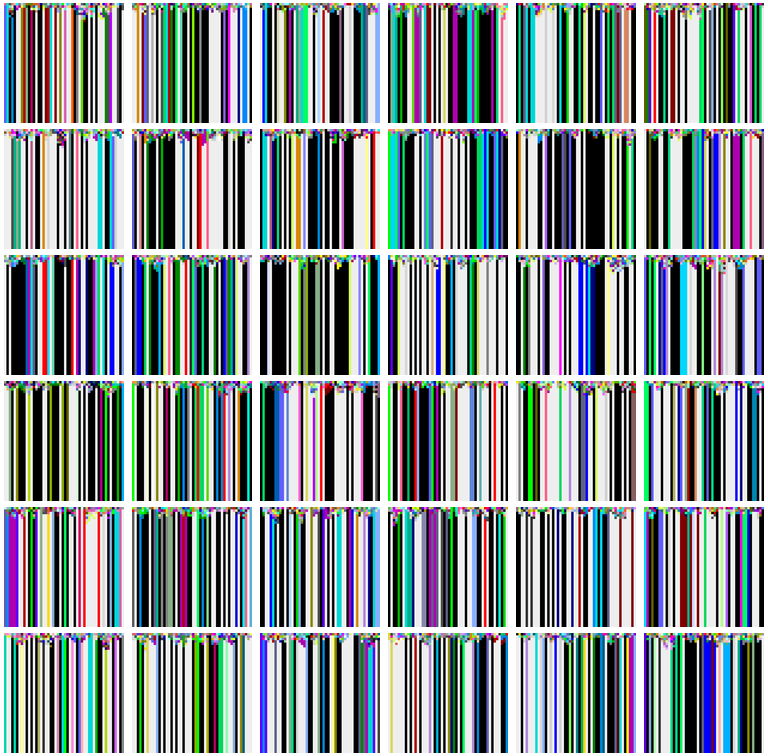
\includegraphics[width=\columnwidth]{paint-drips.png}
\caption{Without the blending rule, things are fairly boring.}
\end{figure}
\clearpage

\section{Results}
(Some pictures can go here).

\begin{figure}

\includegraphics[width=\columnwidth]{flag.png}
\caption{Phenotype with behaviour completely determined by genotype}
\end{figure}

\begin{figure}
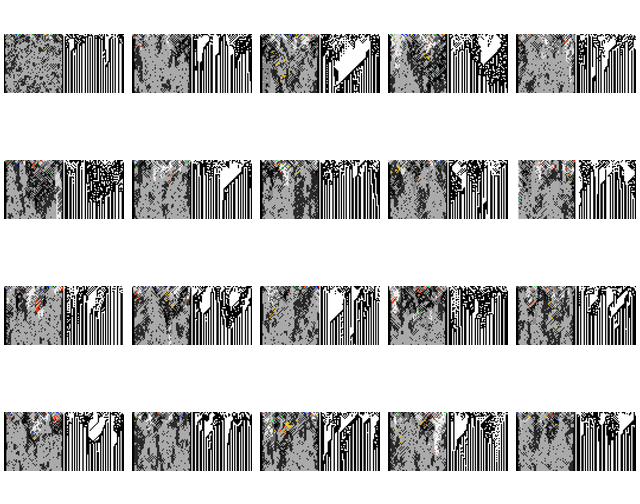
\includegraphics[width=\columnwidth]{baldwin.png}
\caption{Introducing a Baldwin effect}
\end{figure}

\begin{figure}

\includegraphics[width=\columnwidth]{big.png}
\caption{Introducing mutation produces tantalising random structures}
\end{figure}

\begin{figure}
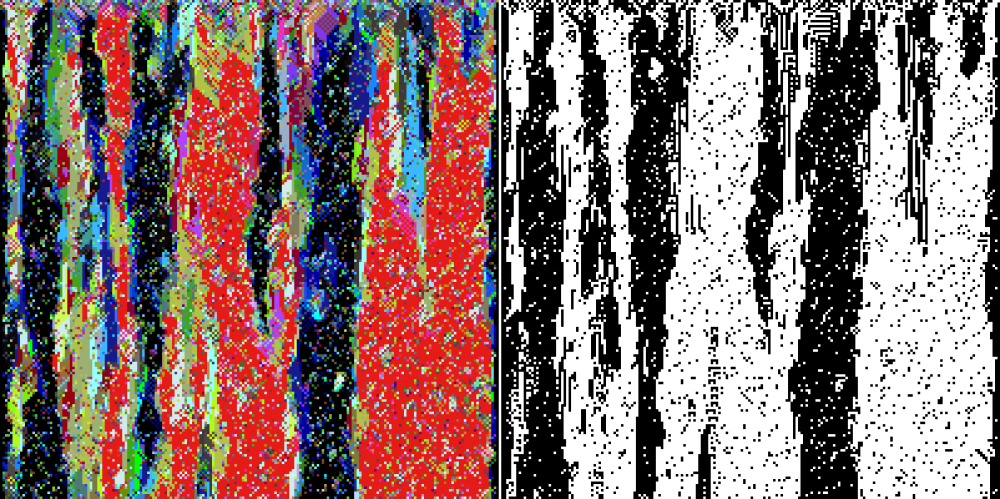
\includegraphics[width=\columnwidth]{lamp-down-low.png}
\caption{Throttling down the mutation rate preserves some of the large-scale stability while making room for variability}
\end{figure}

\begin{figure}

\includegraphics[width=\columnwidth]{eoc.png} \newline
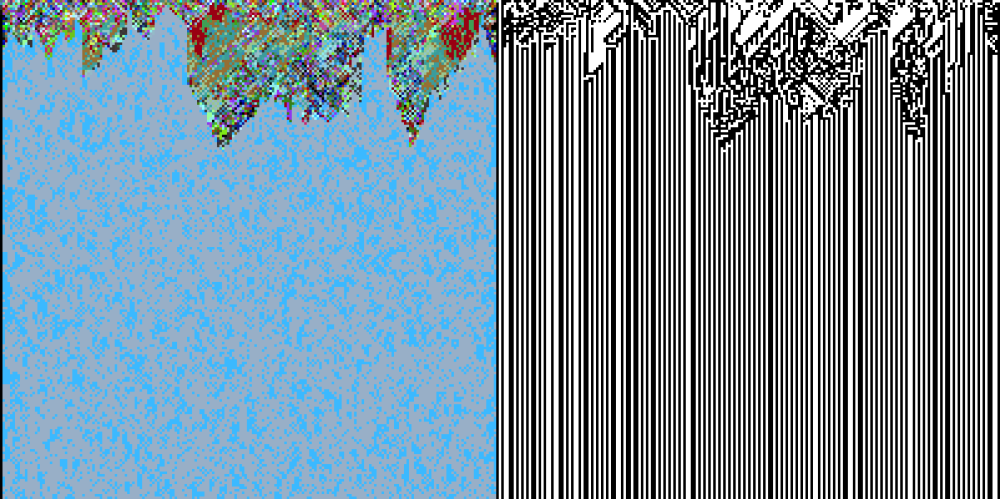
\includegraphics[width=\columnwidth]{reef.png}
\caption{A skewed mutation pattern}
\end{figure}

\begin{figure}
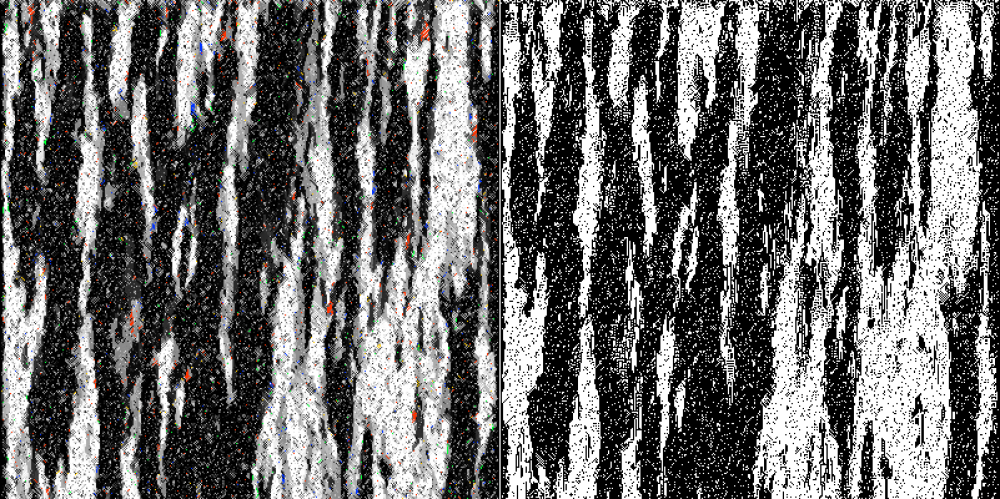
\includegraphics[width=\columnwidth]{seti.png}
\caption{The Search for Intelligent Life in the Universe}
\end{figure}
\clearpage
(Game of life pictures can go here for an interesting comparison
case.)
\newpage

\section{Discussion}

The early experiments seemed provide visual evidence that blending is
a very useful and interesting thing.  Why does it work so well? 

The next set of experiments use a 2-state ``phenotype'' that interacts
with the 256-state ``genotype'' -- or perhaps ``landscape'' or
``ether'' would be a better word.

\clearpage

\section{Conclusion}
% Some of the relevant references are below.
\nocite{*}
We have considerably advanced the field of research.
But much remains to be done.


\section{Acknowledgements}

Coinvent, etc.

\bibliography{metaca}

\end{document}
